\subsubsection*{Design}
As seen in \cref{img:coredes} the core will consist of a block of memory, an ALU combined with the blitter, and several smaller single function cores.
\begin{figure}[H]
	\centering
	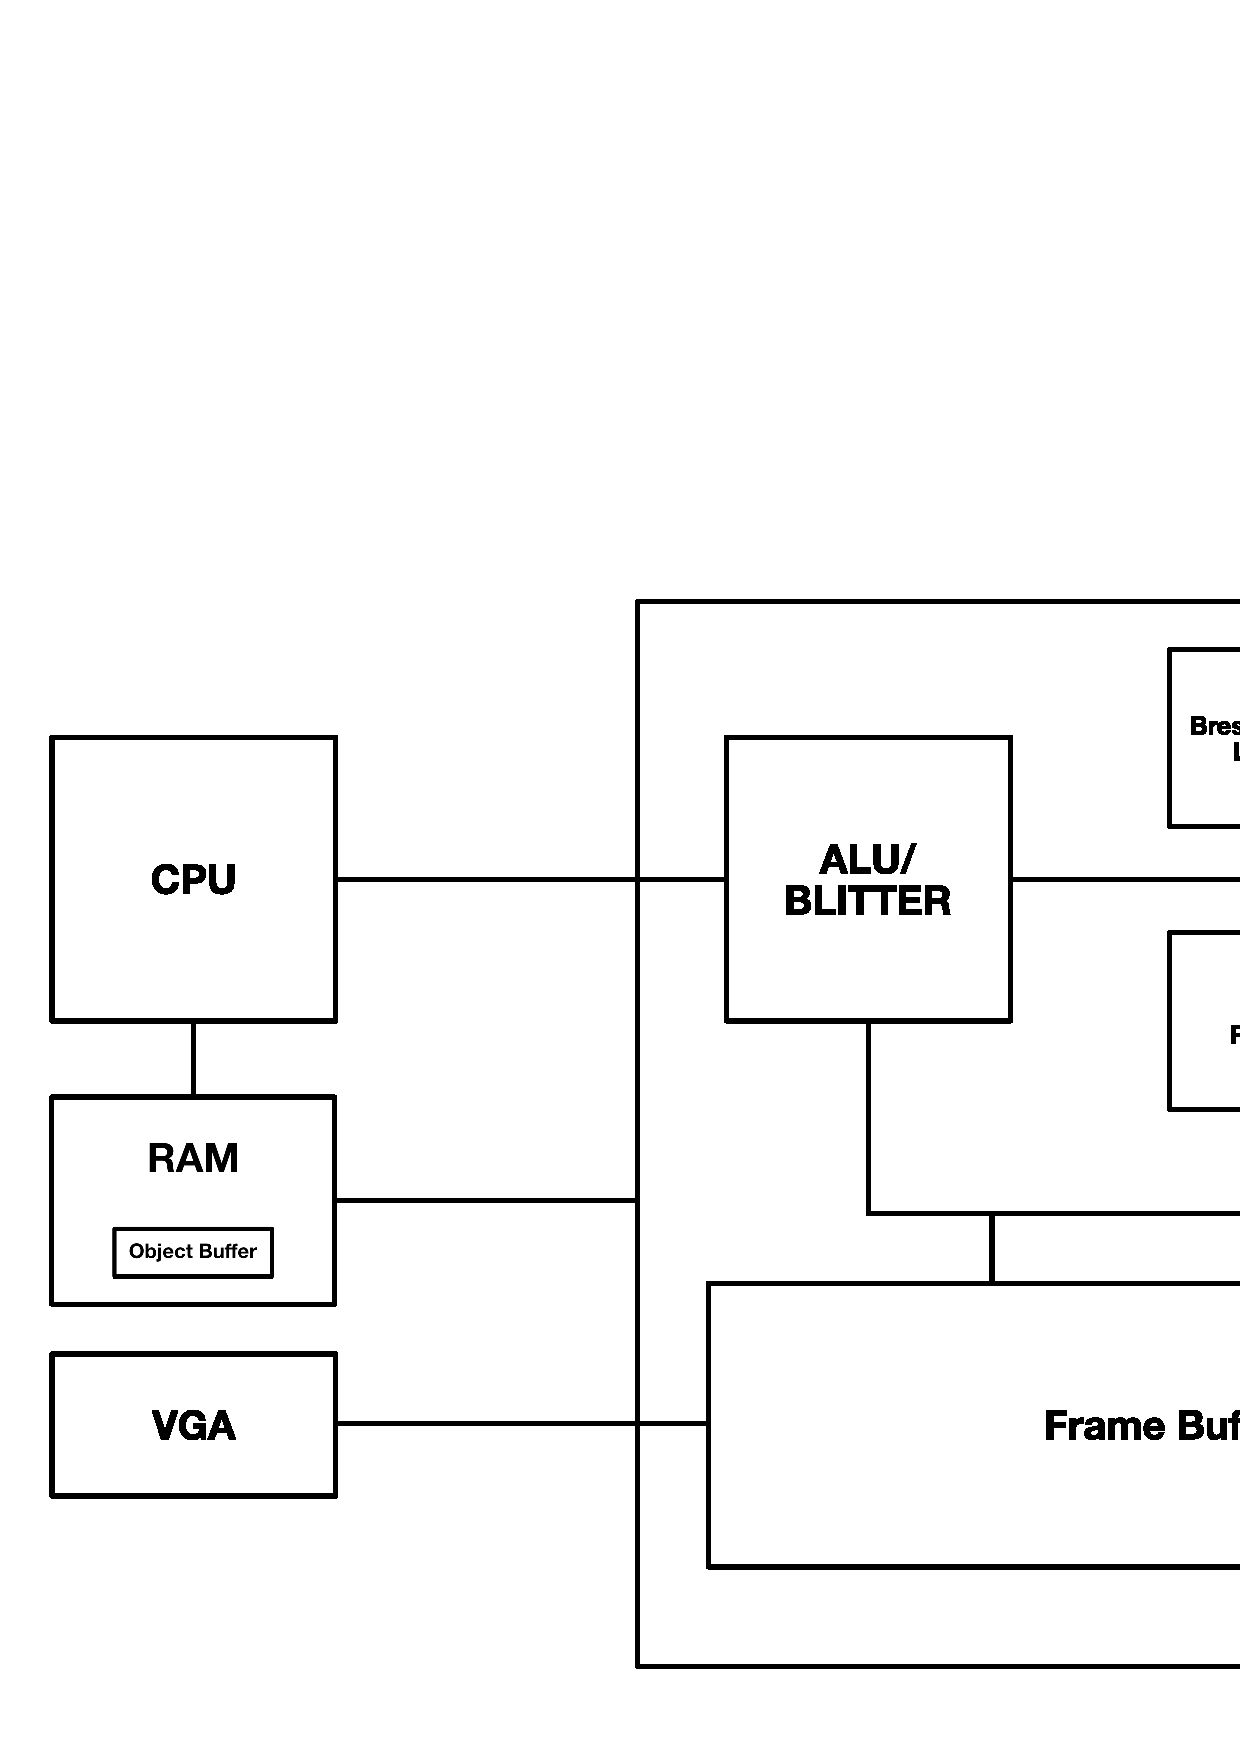
\includegraphics[width=0.5\textwidth]{coredesign}
	\caption{Graphical Design of the AEGIS Core }
	\label{img:coredes}
\end{figure}

The memory will be split up into two parts. The first part consists of the memory for the double frame buffer. It keeps track of the information of two separate frames. One of the frames is drawn by the VGA module, the other is being created by the graphics accelerator and CPU. The other part of the memory is the object memory for the bit blit function. This is needed to know what elements have to be drawn into the frame.

As some functions of the blitter correlate with the functions of the ALU (REFERENCE TO AMIGA MANUAL), the two blocks will be merged together in the following the two of them will be referred to as only the ALU. This part of the core will either write directly into the frame buffer or it will delegate the drawing to the proper function core. These smaller function cores consist of the basic graphical primitives, as discussed in \cref{subsec:des_bresenham}.

For the communication between the CPU and the graphics accelerator, memory mapped registers are going to be used.

\subsubsection*{Implementation}